\documentclass[a4paper,10pt]{report}
\usepackage[utf8]{inputenc}
\usepackage{tikz}
\usetikzlibrary{trees}
\usetikzlibrary{decorations.pathmorphing}
\usetikzlibrary{decorations.markings}

% Title Page
\title{}
\author{Yann Lederrey}

\definecolor{amber}{rgb}{1.0, 0.49, 0.0}
\definecolor{jaune}{rgb}{1.0, 0.75, 0.0}
\definecolor{amethyst}{rgb}{0.6, 0.4, 0.8}
\definecolor{antiquebrass}{rgb}{0.8, 0.58, 0.46}
\definecolor{aqua}{rgb}{0.0, 1.0, 1.0}
\definecolor{babypink}{rgb}{0.96, 0.76, 0.76}

\begin{document}
\maketitle

\tikzset{
    photon/.style={decorate, decoration={snake}, draw=green},
    normal/.style={draw=black}
}
\paragraph{Explication graphiques}
Chaque Noeud cinema correspond au noeud parent du fichier XML.\\
Les noeuds bleu correspondent aux éléments.\\
Les noeuds verts correspondent à des attributs.\\
Les noeuds colorés correspondent à des Id (ID et FK liés selon la couleur).

\begin{center}
\begin{tikzpicture}[
  attribut/.style={rectangle,draw,fill=green!20},
  normal/.style={rectangle,draw,fill=blue!20,rounded corners=.8ex},
  filmid/.style={rectangle,draw,fill=amber!50,rounded corners=.8ex},
  acteurid/.style={rectangle,draw,fill=jaune!50,rounded corners=.8ex},
  genreid/.style={rectangle,draw,fill=amethyst!50,rounded corners=.8ex},
  critiqueid/.style={rectangle,draw,fill=antiquebrass!50,rounded corners=.8ex},
  motcleid/.style={rectangle,draw,fill=aqua!50,rounded corners=.8ex},
  langageid/.style={rectangle,draw,fill=babypink!50,rounded corners=.8ex},
  root/.style={rectangle,draw,fill=red!20},
  transform canvas={scale=0.8},
  sibling distance=7em,]
  \node [root]{cinema}
    child {node[normal] {projections} [normal]
      child { node[normal] {projection} [normal]
	child { node[normal] {dateProjection} [normal]}
	child { node[normal] {numeroSalle} [normal]}
	child { node[normal] {filmProj} [normal]
	  child { node[filmid] {filmId} [normal]}
	  }
	child { node[normal] {acteursProj} [normal]
	  child { node[acteurid] {acteurProj} [normal]
	    child { node[attribut] {acteurProjId} [normal]}
	    child { node[attribut] {nomRole} [normal]}
	    child { node[attribut] {placeRole} [normal]}
	  }
	}
      }
    };
\end{tikzpicture}
\end{center}

\vspace{170px}

\begin{center}
\begin{tikzpicture}[
  attribut/.style={rectangle,draw,fill=green!20},
  normal/.style={rectangle,draw,fill=blue!20,rounded corners=.8ex},
  filmid/.style={rectangle,draw,fill=amber!50,rounded corners=.8ex},
  acteurid/.style={rectangle,draw,fill=jaune!50,rounded corners=.8ex},
  genreid/.style={rectangle,draw,fill=amethyst!50,rounded corners=.8ex},
  critiqueid/.style={rectangle,draw,fill=antiquebrass!50,rounded corners=.8ex},
  motcleid/.style={rectangle,draw,fill=aqua!50,rounded corners=.8ex},
  langageid/.style={rectangle,draw,fill=babypink!50,rounded corners=.8ex},
  root/.style={rectangle,draw,fill=red!20},
  transform canvas={scale=0.8},
  sibling distance=7em,]
  \node [root]{cinema}
  child {node[normal] {films} [normal]
    child { node[normal] {film} [normal]
      child { node[filmid] {filmId} [normal]}
      child { node[normal] {titre} [normal]}
      child { node[normal] {synopsis} [normal]}
      child { node[normal] {duree} [normal]}
      child { node[normal] {critiqueFilm} [normal]
	child { node[critiqueid] {critiquesFilmId} [normal]}
      }
      child { node[normal] {genresFilm} [normal]
	child { node[normal] {genreFilm} [normal]
	  child { node[genreid] {genreFilmId} [normal]}
	}
      }
      child { node[normal] {motsCleFilm} [normal]
	child { node[normal] {motCleFilm} [normal]
	  child { node[motcleid] {motCleFilmId} [normal]}
	}
      }
      child { node[normal] {langagesFilm} [normal]
	child { node[normal] {langageFilm} [normal]
	  child { node[langageid] {langageFilmId} [normal]}
	  }
	}
      child { node[normal] {photo} [normal]}
    }
  };
\end{tikzpicture}
\end{center}

\vspace{170px}

\begin{center}
\begin{tikzpicture}[
  attribut/.style={rectangle,draw,fill=green!20},
  normal/.style={rectangle,draw,fill=blue!20,rounded corners=.8ex},
  filmid/.style={rectangle,draw,fill=amber!50,rounded corners=.8ex},
  acteurid/.style={rectangle,draw,fill=jaune!50,rounded corners=.8ex},
  genreid/.style={rectangle,draw,fill=amethyst!50,rounded corners=.8ex},
  critiqueid/.style={rectangle,draw,fill=antiquebrass!50,rounded corners=.8ex},
  motcleid/.style={rectangle,draw,fill=aqua!50,rounded corners=.8ex},
  langageid/.style={rectangle,draw,fill=babypink!50,rounded corners=.8ex},
  root/.style={rectangle,draw,fill=red!20},
  transform canvas={scale=0.8},
  sibling distance=7em,]
  \node [root]{cinema}
   child { node[normal] {acteurs} [normal]
    child { node[normal] {acteur} [normal]
      child { node[acteurid] {acteurId} [normal]}
      child { node[normal] {nom} [normal]}
      child { node[normal] {nomNaissance} [normal]}
      child { node[normal] {biographie} [normal]}
      child { node[normal] {sexe} [normal]
	child { node[attribut] {type(enum)} [normal]}
      }
      child { node[normal] {dateNaissance} [normal]}
      child { node[normal] {dateDeces} [normal]}
    }
   };
\end{tikzpicture}
\end{center}

\vspace{170px}

\begin{center}
\begin{tikzpicture}[
  attribut/.style={rectangle,draw,fill=green!20},
  normal/.style={rectangle,draw,fill=blue!20,rounded corners=.8ex},
  filmid/.style={rectangle,draw,fill=amber!50,rounded corners=.8ex},
  acteurid/.style={rectangle,draw,fill=jaune!50,rounded corners=.8ex},
  genreid/.style={rectangle,draw,fill=amethyst!50,rounded corners=.8ex},
  critiqueid/.style={rectangle,draw,fill=antiquebrass!50,rounded corners=.8ex},
  motcleid/.style={rectangle,draw,fill=aqua!50,rounded corners=.8ex},
  langageid/.style={rectangle,draw,fill=babypink!50,rounded corners=.8ex},
  root/.style={rectangle,draw,fill=red!20},
  transform canvas={scale=0.8},
      level 1/.style={sibling distance=6cm},
    level 2/.style={sibling distance=3cm}, 
    level 3/.style={sibling distance=2cm},]
  \node [root]{cinema}
  child { node[normal] {motsCleFilm} [normal]
    child { node[normal] {motCle} [normal]
      child { node[motcleid] {motCleId} [normal]}
      child { node[normal] {labelMc} [normal]}
    }
  }
  child { node[normal] {genres} [normal]
      child { node[normal] {genre} [normal]
      child { node[genreid] {genreId} [normal]}
      child { node[normal] {labelGe} [normal]}
    }
  }
  child { node[normal] {langages} [normal]
    child { node[normal] {langage} [normal]
    child { node[langageid] {langageId} [normal]}
      child { node[normal] {labelLa} [normal]}
    }
  }
  child { node[normal] {critiques} [normal]
    child { node[normal] {critique} [normal]
      child { node[critiqueid] {critiqueId} [normal]}
      child { node[normal] {texte} [normal]}
      child { node[normal] {note} [normal]}
    }
  };
\end{tikzpicture}
\end{center}


\end{document}          
